\RequirePackage[T1]{fontenc}
\documentclass[conference,letterpaper]{IEEEtran}
\usepackage{amsmath,amssymb,graphicx,booktabs,array,tabularx,url}
\usepackage{balance}
\usepackage[hidelinks]{hyperref}
\hypersetup{pdftitle={Memorization and Generalization under Training-Label Randomization on Tabular Data},pdfauthor={Tianying Chen, Linjie Yang, Elsey Chen},pdfsubject={ECS 171 Group 8; technical report review version, October 18, 2026},pdfkeywords={label randomization, Dry Bean, memorization, generalization, reproducibility}}
\graphicspath{{figures/}}
\newcommand{\meanstd}[2]{\ensuremath{#1\,\mathord{\pm}\,#2}}
\newcommand{\code}[1]{\texttt{#1}}
\newcolumntype{L}[1]{>{\raggedright\arraybackslash}p{#1}}
\setlength{\emergencystretch}{1em}
\pagestyle{plain}
\raggedbottom
\begin{document}
\title{Memorization and Generalization under\\
Training-Label Randomization on Tabular Data}
\author{\IEEEauthorblockN{Tianying Chen, Linjie Yang, and Elsey Chen}
\IEEEauthorblockA{Department of Computer Science, University of California, Davis\\
ECS 171, Group 8\\
\{tiaychen, yljyang, elschen\}@ucdavis.edu}}
\maketitle

\begin{abstract}
Accurate predictions on training examples can reflect either transferable structure or memorization of the supplied answers. Inspired by random-label experiments in deep learning, we compare these behaviors across three model families on the UCI Dry Bean dataset. After exact deduplication, we use 13,543 observations, 16 numerical features, seven classes, and one fixed stratified train/validation/test split. Ten clean-label candidate fits select hyperparameters before 45 fresh main fits: logistic regression (LR), random forest (RF), and a multilayer perceptron (MLP), each evaluated at five training-label randomization probabilities and three paired seeds. Validation and test labels remain clean. Clean-label test Macro-F1 is 0.9404 for LR, 0.9361 for RF, and 0.9346 for MLP. Under complete random-label replacement, RF fits the supplied training labels perfectly but reaches only 0.1314 clean-test Macro-F1. The finite-budget MLP fits 38.06\% of randomized training labels, with test Macro-F1 0.1309; LR reaches 0.1144. At partial randomization, model responses differ substantially: at $p=0.75$, LR retains 0.9073 Macro-F1, compared with 0.6440 for RF and 0.5856 for MLP. These results separate random-label fitting from useful prediction within this dataset and protocol. We provide saved predictions, integrity records, reproducible figure generation, and a hosted web inference interface. Three seeds on one split describe conditional run variation, not statistical significance or cross-dataset superiority.
\end{abstract}
\begin{IEEEkeywords}
label noise, memorization, generalization, tabular classification, reproducibility
\end{IEEEkeywords}

\section{Introduction}
\label{sec:introduction}
A supervised classifier learns from input--label pairs, but a high training score does not identify what it has learned. A flexible model may associate each training input with an arbitrary answer rather than recover a relationship that also holds for new inputs. Label randomization makes this distinction observable: the inputs stay unchanged while some training answers are replaced, and evaluation still asks for the original categories on unseen examples. Success at fitting the altered answers and success at predicting the underlying categories become separate measurements.

Zhang et al.~\cite{zhang2017rethinking} demonstrate that selected image-classification networks can fit random labels nearly or perfectly. Their experiments challenge explanations that rely only on explicit regularization or a model's ability to fit the training set. They do not imply that every neural network will memorize every finite dataset under any optimizer, regularization strength, or training budget. This distinction matters when applying their motivation to a smaller course project with a different data representation.

We investigate seven-class classification using numerical measurements extracted from dry-bean images. The learning inputs are the supplied tabular features; our models do not process images or extract features from pixels. We compare a linear classifier, a tree ensemble, and a feedforward neural network. This setup makes model-family differences visible while keeping the dataset, split, label perturbations, and evaluation targets controlled.

Our two research questions are:
\begin{itemize}
\item \textbf{RQ1:} How does training-label randomization affect clean-test Macro-F1 across logistic regression, random forest, and an MLP?
\item \textbf{RQ2:} Does stronger agreement with randomized training labels coincide with better predictions of original labels on unseen observations?
\end{itemize}

The primary comparison fixes hyperparameters selected on clean labels. We therefore measure how established clean-data configurations respond to progressively less informative supervision. We do not optimize a separate noise-aware model at every perturbation level, nor estimate the best achievable robustness of any model family.

The project makes three concrete contributions. First, it implements a paired randomization experiment with an explicit distinction between the probability of redrawing a label and the fraction that actually changes. Second, it reports training agreement with both supplied and original labels alongside clean-test metrics, preventing increased fitting capacity from being confused with generalization. Third, it links the analysis to saved per-observation predictions, frozen experiment records, and a web interface that uses the same saved preprocessing and models.

This report describes completed core experiments and verified public deployment as of October 18, 2026. The final section separates delivered artifacts from remaining team acceptance and presentation work. No additional configurations were selected from the reported test results.

\section{Background and Related Work}
\label{sec:related}
\subsection{Random Labels as a Diagnostic}
The assigned paper studies what happens when the association between inputs and labels is deliberately destroyed~\cite{zhang2017rethinking}. If a sufficiently flexible learner can still fit the training data, small training error alone cannot certify that it learned a useful input--output relationship. Its random-label experiments, finite-sample expressivity results, and discussion of implicit regularization address related but different questions. An existence result for a network representing arbitrary labels is not a guarantee that a particular optimization run will find that representation.

Arpit et al.~\cite{arpit2017memorization} further examine memorization and learning dynamics in deep networks. Their findings motivate recording optimization behavior rather than treating all networks as equivalent black boxes. Our saved MLP loss curves and stopping records support a bounded statement about the network actually trained. They do not recover the original papers' image experiments, architecture search, or theoretical claims.

\subsection{Tabular Classification and Model Families}
Dry Bean was introduced as a multiclass dataset based on computer-vision measurements~\cite{koklu2020drybeans,uci2020drybean}. Its continuous size and shape variables provide a compact alternative to the high-dimensional image inputs used in the assigned paper. The original Dry Bean study uses a different evaluation protocol, including cross-validation and accuracy. Its headline performance is therefore not a directly comparable benchmark for our deduplicated fixed-split Macro-F1 results.

Random forests aggregate randomized decision trees~\cite{breiman2001randomforests}. The selected unrestricted-depth forest can fit highly specific partitions, making its training behavior useful for a memorization comparison. Logistic regression provides a regularized linear decision rule after standardization. The MLP supplies nonlinear learned representations, trained with Adam~\cite{kingma2015adam}. All three estimators use scikit-learn~\cite{pedregosa2011scikit}, allowing consistent preprocessing, metrics, and serialization.

Our contribution is an empirical comparison under one controlled tabular protocol. It is not a new noise-correction algorithm, a reproduction of image-network results, or a claim that linear models generally outperform neural or tree-based methods. The modest dataset and computation budget make the experiment inspectable but also restrict its scope.

\section{Dataset and Exploratory Analysis}
\label{sec:data}
\subsection{Source, Audit, and Split}
The UCI release contains 13,611 observations, 16 numerical predictors, and seven bean classes~\cite{uci2020drybean}. We preserve the original archive and workbook and record their hashes. The audit finds no missing or nonfinite feature values, 68 exactly duplicated rows, and no feature-identical groups with conflicting labels. All 68 removed duplicates belong to HOROZ. Keeping the first occurrence leaves 13,543 distinct rows.

Deduplication precedes splitting to prevent identical observations from appearing in both training and evaluation partitions. The resulting evaluation population is the set of distinct supplied rows, not the original frequency-weighted collection with duplicates. This decision changes the HOROZ count from 1,928 to 1,860. We retain an original workbook row identifier for traceability and never use it as a predictor.

We first reserve 20\% of cleaned data for testing using stratification and random state 171. A second stratified split, with random state 172, reserves 25\% of the remainder for validation. Final sizes are 8,125 training, 2,709 validation, and 2,709 test observations. Table~\ref{tab:classcounts} gives exact class counts. Stratification preserves approximate class proportions; it does not create equal class sizes or establish independence among biologically related samples.

\begin{table}[t]
\caption{Class counts after deduplication and in the fixed split.}
\label{tab:classcounts}
\centering\small
\begin{tabular}{lrrrr}
\toprule
Class & Cleaned & Train & Val. & Test\\
\midrule
BARBUNYA & 1,322 & 793 & 264 & 265\\
BOMBAY & 522 & 313 & 105 & 104\\
CALI & 1,630 & 978 & 326 & 326\\
DERMASON & 3,546 & 2,127 & 710 & 709\\
HOROZ & 1,860 & 1,116 & 372 & 372\\
SEKER & 2,027 & 1,216 & 405 & 406\\
SIRA & 2,636 & 1,582 & 527 & 527\\
\midrule
Total & 13,543 & 8,125 & 2,709 & 2,709\\
\bottomrule
\end{tabular}
\end{table}

\subsection{Feature Structure and Class Imbalance}
Exploratory analysis uses only the training partition. The largest training class, DERMASON, contains 2,127 observations, whereas BOMBAY contains 313, a ratio of 6.80. A metric dominated by the largest classes could conceal poor performance on smaller ones. We therefore use Macro-F1 as the primary measure and include balanced accuracy and class-specific results.

The predictors describe related aspects of geometry. Area, ConvexArea, Perimeter, and EquivDiameter capture size; major and minor axis lengths describe extent along principal directions. Aspect ratio, eccentricity, compactness, roundness, solidity, extent, and four shape factors encode normalized shape information. We preserve the release's spelling, including \code{AspectRation} and lowercase \code{roundness}, so the feature schema remains consistent from the workbook to the inference interface.

Figure~\ref{fig:eda} shows class imbalance and the wide range of feature scales. A numerical difference of one unit has very different meaning for an area measure and a normalized shape descriptor. LR and MLP therefore use a StandardScaler fitted exclusively on training inputs. No validation or test observations enter its mean or variance estimates. RF uses the original numerical values.

\begin{figure*}[t]
\centering
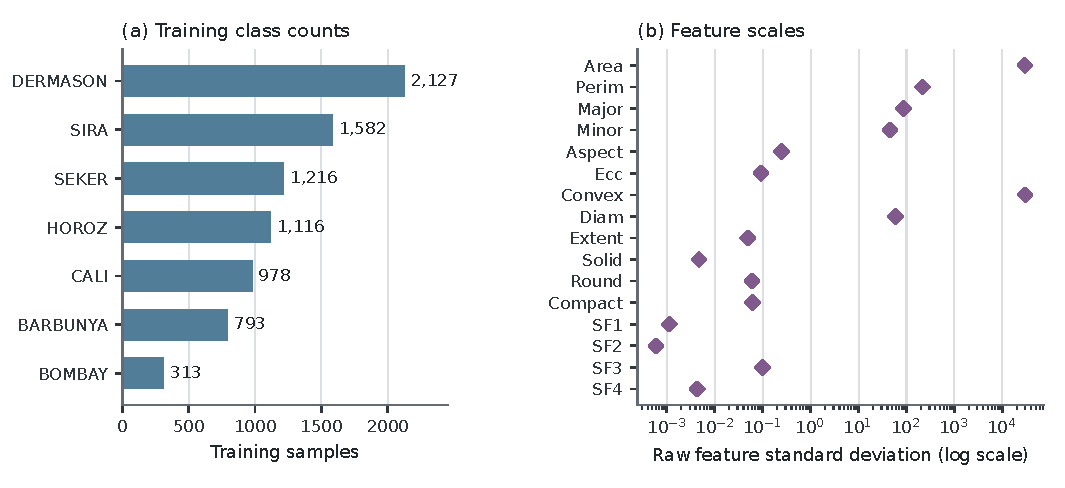
\includegraphics[width=\textwidth]{eda_class_scale.pdf}
\caption{Training-only exploratory analysis ($n=8{,}125$). Class counts reveal imbalance; raw feature standard deviations illustrate scale differences. A logarithmic scale is used only for the scale summary, not as a transformation applied to model inputs. Source: saved training partition and EDA tables.}
\label{fig:eda}
\end{figure*}

Several predictors are strongly correlated (Fig.~\ref{fig:correlation}). Area and ConvexArea have Pearson $r=0.999940$; Compactness and ShapeFactor3 have $r=0.998683$; Perimeter and EquivDiameter have $r=0.991365$. The 16 columns should not be interpreted as 16 independent sources of information. These dependencies also make individual linear coefficients difficult to interpret causally.

We retain all 16 original features according to the fixed design. There is no test-driven feature deletion, PCA, or skewness transformation. Observations that appear extreme in a distribution plot are retained; hiding fliers in an exploratory boxplot affects the display only. The experiment studies label randomization, so changing feature engineering across noise levels would introduce an additional intervention.

\begin{figure*}[t]
\centering
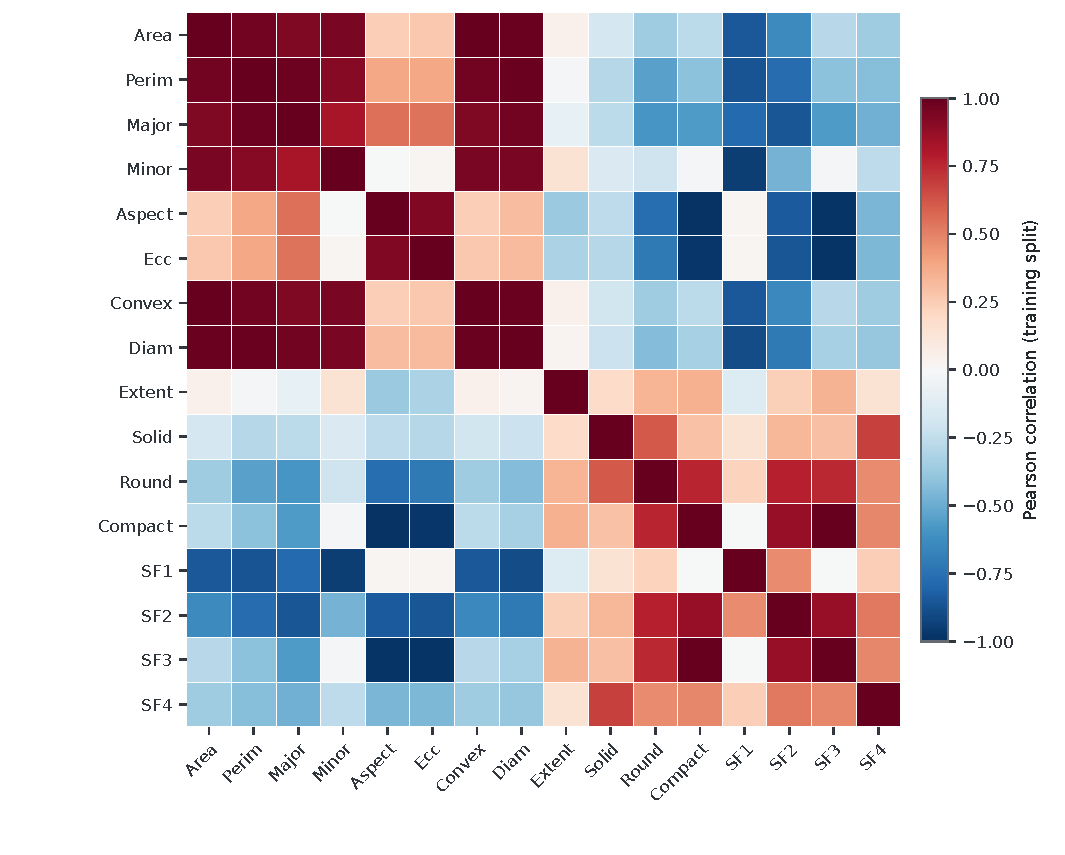
\includegraphics[width=0.92\textwidth]{eda_correlation.pdf}
\caption{Pearson correlations on training inputs only. Perim, Major/Minor, Ecc, Convex, Diam, Solid, Round, and Compact abbreviate the corresponding size/shape features; SF1--SF4 denote the four shape factors. Strong correlations motivate caution in coefficient interpretation and are not used for test-driven feature selection.}
\label{fig:correlation}
\end{figure*}

\subsection{Data Boundaries}
The source provides class labels and extracted measurements rather than a collection protocol designed for our robustness question. We have no independent acquisition-site or batch identifiers for a grouped split. A random stratified split supports an in-dataset comparison but cannot establish transfer to new harvests, devices, laboratories, or growing conditions. The web interface accepts numerical descriptors; it does not identify beans directly from photographs.

\section{Experimental Methodology}
\label{sec:methods}
\subsection{Label-Randomization Mechanism}
Let $(x_i,y_i)$ denote a training observation with $y_i\in\{1,\ldots,K\}$ and $K=7$. For replicate seed $s$, we draw independent $u_i\sim\mathcal{U}[0,1)$ and $z_i\sim\operatorname{Uniform}\{1,\ldots,K\}$. At randomization level $p$, the supplied training label is
\begin{equation}
\widetilde y_i^{(p,s)}=
\begin{cases}
z_i,&u_i<p,\\
y_i,&u_i\ge p.
\end{cases}
\label{eq:noise}
\end{equation}
The redraw can return the original class. The expected actual changed-label fraction is therefore
\begin{equation}
\mathbb{E}[q(p,s)]=p\left(1-\frac{1}{K}\right)=\frac{6p}{7}.
\label{eq:changed}
\end{equation}
Thus $p=1$ means every label is independently redrawn, not that every resulting label differs from its original value. The expected changed fraction is 85.71\%; the observed three-seed mean is 85.93\%. We record realized $q$ instead of silently treating it as equal to $p$.

For each seed, the same vectors $u$ and $z$ are reused across $p\in\{0,0.25,0.50,0.75,1\}$. Increasing $p$ adds selected observations within a nested intervention. All models receive exactly the same perturbed label vector at a given $(p,s)$. A label vector remains fixed throughout its fit; labels are not redrawn between epochs. Validation and test labels remain unchanged at every condition.

The replacement transition matrix is
\begin{equation}
T(p)=(1-p)I+\frac{p}{K}\mathbf{1}\mathbf{1}^{\mathsf{T}}.
\label{eq:transition}
\end{equation}
This defines independent uniform replacement noise. It does not model realistic annotation errors that depend on class, image ambiguity, or feature values.

\subsection{Models and Clean-Label Selection}
Table~\ref{tab:models} summarizes the candidate grids and selected settings. LR uses an L2 penalty, LBFGS, a maximum of 2,000 iterations, and tolerance $10^{-4}$. RF uses 200 trees, bootstrap sampling, and square-root feature subsampling. The selected forest has unrestricted depth and one observation per minimum leaf. Class weights remain unset for all models.

The MLP has architecture $16\!\rightarrow\!128\!\rightarrow\!64\!\rightarrow\!7$, ReLU hidden activations, and 10,887 trainable weights and biases. It uses Adam, batch size 128, initial learning rate $10^{-3}$, and at most 500 iterations. The tolerance is $10^{-5}$ with 20 iterations without sufficient improvement. Explicit validation-based early stopping is disabled; the estimator's training-objective stopping rule still applies. The selected L2 parameter is $\alpha=0.01$.

\begin{table}[t]
\caption{Ten clean-label candidate fits, all with seed 17. Bold settings are selected before the main experiment.}
\label{tab:models}
\centering\footnotesize
\begin{tabular}{L{0.35in}L{1.80in}r}
\toprule
Model & Candidates / selected setting & Val. F1\\
\midrule
LR & $C=0.1$ & 0.9316\\
   & $\mathbf{C=1}$ & \textbf{0.9328}\\
   & $C=10$ & 0.9320\\
\midrule
RF & depth 8, leaf 1 & 0.9162\\
   & depth 8, leaf 5 & 0.9172\\
   & \textbf{unlimited depth, leaf 1} & \textbf{0.9239}\\
   & unlimited depth, leaf 5 & 0.9217\\
\midrule
MLP & $\alpha=0$ & 0.9299\\
    & $\alpha=0.0001$ & 0.9276\\
    & $\boldsymbol{\alpha=0.01}$ & \textbf{0.9331}\\
\bottomrule
\end{tabular}
\end{table}

Selection uses clean validation Macro-F1 exclusively. Candidates within 0.001 of the best score are tied; deterministic preferences are smaller $C$ for LR, shallower depth then larger leaves for RF, and larger $\alpha$ for MLP. Candidate values, tie rules, selected configurations, the split, and the main matrix are stored before accessing test results. This is a small, transparent search rather than exhaustive optimization.

Each main model is initialized and fitted anew. We use seeds 17, 29, and 43 for both label randomization and the estimator's random state. Pairing controls labels across model families but changes data perturbation and model randomness together. It does not separately identify their variance components.

\subsection{Evaluation Targets and Metrics}
The main endpoint is clean-test Macro-F1. Seven labels are included explicitly, with undefined per-class F1 set to zero:
\begin{equation}
F_{1,\mathrm{macro}}=\frac{1}{K}\sum_{k=1}^{K}
\frac{2\operatorname{TP}_k}{2\operatorname{TP}_k+\operatorname{FP}_k+\operatorname{FN}_k}.
\label{eq:macro}
\end{equation}
The zero-denominator convention applies when a fraction is undefined. We also report accuracy, balanced accuracy (mean class recall), class-specific scores, fit time, and convergence information.

For training inputs, two accuracies answer different questions:
\begin{align}
A_{\mathrm{train,noisy}}&=\frac{1}{n}\sum_i
\mathbf{1}[f(x_i)=\widetilde y_i],\\
A_{\mathrm{train,clean}}&=\frac{1}{n}\sum_i
\mathbf{1}[f(x_i)=y_i].
\end{align}
Here $\mathbf{1}[\cdot]$ is the indicator function. The first accuracy measures agreement with supplied supervision; the second measures agreement with original labels on the same inputs. Comparing $A_{\mathrm{train,noisy}}$ with clean-test accuracy mixes targets. We do not call their difference a standard generalization gap. A separately stored clean-target difference uses $A_{\mathrm{train,clean}}-A_{\mathrm{test,clean}}$. Since training uses altered targets, that difference may be negative without indicating leakage or an arithmetic error.

The clean-training majority class is DERMASON. Always predicting it gives test accuracy 0.2617, balanced accuracy 0.1429, and Macro-F1 0.0593. Independently uniform random predictions have expected accuracy $1/7$; this is not a universal Macro-F1 baseline or a value every random-label-trained classifier must attain. We use no horizontal ``chance'' line on Macro-F1 plots.

For each model--noise condition, we report the arithmetic mean and sample standard deviation over three runs. Error bars describe variation conditional on the fixed split and joint randomization scheme. They are not confidence intervals, do not reflect new splits, and do not justify significance or universal-superiority claims.

\subsection{Execution Order and Integrity}
The main matrix contains 45 fits; the ten selection fits bring the research total to 55. Historical smoke runs and superseded pre-review outputs are excluded from this research set. The selected configuration was frozen at 05:31:45 UTC on October 13, 2026, before final holdout evaluation at 05:39:35 UTC. These are execution timestamps; the report snapshot is October 18 in the course's local time zone.

Source and data hashes, split identities, package versions, and per-run metadata accompany the artifacts. The evaluation gate checks the frozen context and completion of the predeclared matrix before reading the test partition. Stored per-observation predictions permit independent metric recomputation without fitting models again. A read-only report audit recomputed training and validation scores for all 55 fits, test scores for all 45 main fits, and all 15 summary means and sample standard deviations.

The holdout has now been revealed. Any subsequent capacity experiment, preprocessing change, or model configuration must be labeled exploratory instead of being silently folded into the original matrix.

\section{Experimental Results}
\label{sec:results}
\subsection{Overall Clean-Test Performance}
Table~\ref{tab:main} and Fig.~\ref{fig:performance} answer RQ1. With clean training labels, test Macro-F1 is 0.9404 for LR, 0.9361 for RF, and 0.9346 for MLP. Their clean-test accuracies are 0.9280, 0.9256, and 0.9210. The numerical ordering describes this split and these settings; the small differences are not evidence of a general ranking.

\begin{table*}[t]
\caption{Clean-test Macro-F1 under training-label randomization. Entries are mean $\pm$ sample SD over three seeds on the same split. Actual changed fraction $q$ is shared across models.}
\label{tab:main}
\centering\small
\begin{tabular}{ccccc}
\toprule
Redraw probability $p$ & Actual changed fraction $q$ & LR & RF & MLP\\
\midrule
0.00 & \meanstd{0.0000}{0.0000} & \meanstd{0.9404}{0.0000} & \meanstd{0.9361}{0.0012} & \meanstd{0.9346}{0.0040}\\
0.25 & \meanstd{0.2156}{0.0052} & \meanstd{0.9164}{0.0028} & \meanstd{0.9280}{0.0047} & \meanstd{0.9029}{0.0024}\\
0.50 & \meanstd{0.4306}{0.0071} & \meanstd{0.9112}{0.0029} & \meanstd{0.8767}{0.0014} & \meanstd{0.8391}{0.0094}\\
0.75 & \meanstd{0.6486}{0.0078} & \meanstd{0.9073}{0.0044} & \meanstd{0.6440}{0.0219} & \meanstd{0.5856}{0.0419}\\
1.00 & \meanstd{0.8593}{0.0058} & \meanstd{0.1144}{0.0552} & \meanstd{0.1314}{0.0205} & \meanstd{0.1309}{0.0172}\\
\bottomrule
\end{tabular}
\end{table*}

\begin{figure*}[t]
\centering
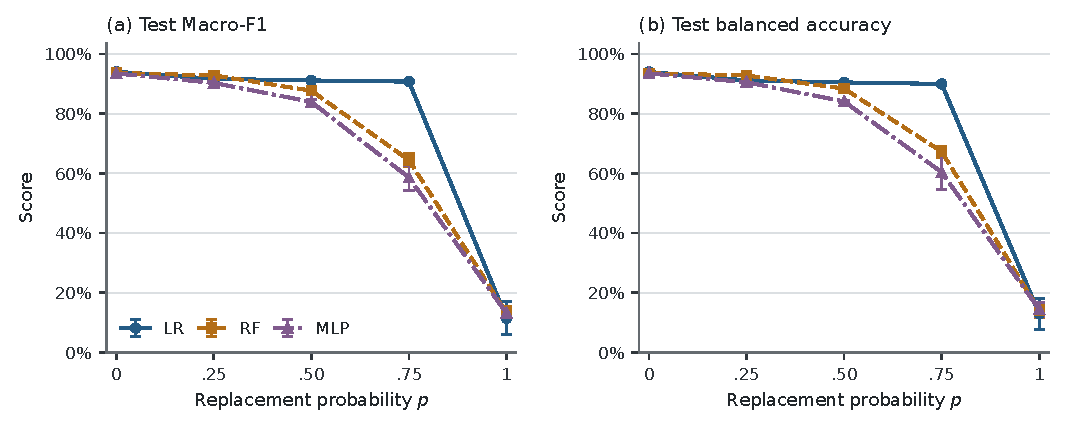
\includegraphics[width=\textwidth]{test_performance.pdf}
\caption{Clean-test Macro-F1 and balanced accuracy versus training-label redraw probability. Points are three-seed means; bars show sample SD, not confidence intervals. All conditions use the same 2,709 test observations with original labels. Lines connect the five measured conditions and do not establish behavior at unmeasured levels.}
\label{fig:performance}
\end{figure*}

At $p=0.25$, RF retains mean Macro-F1 0.9280, compared with 0.9164 for LR and 0.9029 for MLP. At stronger perturbations the ordering changes. LR reaches 0.9112 at $p=0.50$ and 0.9073 at $p=0.75$, while RF falls to 0.8767 and 0.6440 and MLP to 0.8391 and 0.5856. Relative to their clean-label baselines, the $p=0.75$ drops are 0.0331, 0.2921, and 0.3490 Macro-F1 units for LR, RF, and MLP.

Complete replacement produces a much larger decline for every model. At $p=1$, means range from 0.1144 to 0.1314. Balanced accuracy falls to 0.1291 for LR, 0.1407 for RF, and 0.1436 for MLP. This secondary metric supports degradation across classes rather than only through one aggregate weighting.

LR's zero SD at $p=0$ has a specific explanation: labels and the split are identical and LBFGS follows the same deterministic fit. Three seed values do not create three independent clean datasets. At $p=1$, its Macro-F1 SD rises to 0.0552, the largest endpoint variation among the three models. Stable performance at moderate replacement levels should not be described as stability under all noise conditions.

\subsection{Training Agreement and Memorization}
Figure~\ref{fig:targets} and Table~\ref{tab:endpoint} answer RQ2. RF obtains 100\% training accuracy against supplied labels at all five levels. As $p$ increases, its original-label training accuracy declines with the fraction that changed: a model reproducing every supplied answer also reproduces deliberately introduced errors. At complete replacement, its mean original-label training accuracy is 0.1407 and clean-test accuracy is 0.1378.

\begin{figure*}[t]
\centering
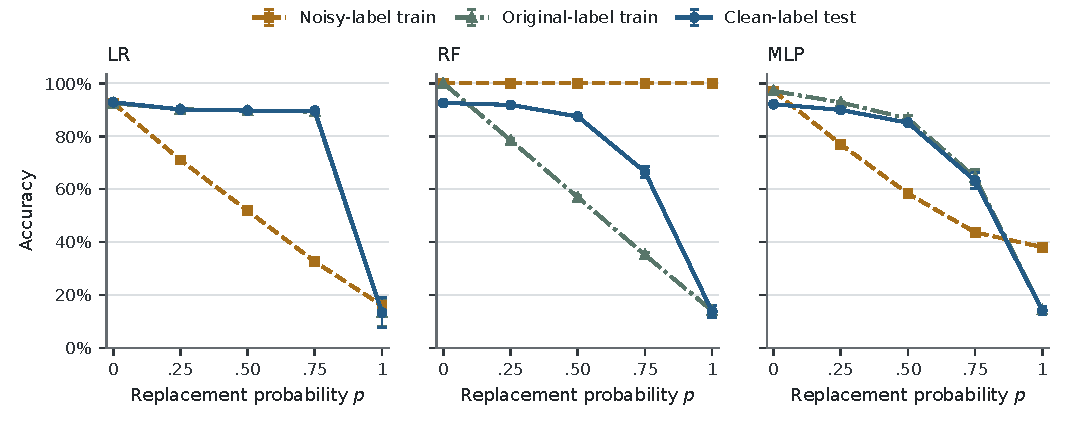
\includegraphics[width=\textwidth]{fitting_targets.pdf}
\caption{Three distinct accuracy targets for each model: supplied training labels, original training labels, and original test labels. Means and sample SD use the same three seeds. Noisy-training and clean-test curves compare different targets; their separation is not a conventional generalization gap. RF's perfect supplied-label fit persists even as clean-test prediction deteriorates.}
\label{fig:targets}
\end{figure*}

\begin{table}[t]
\caption{Endpoint behavior at $p=1$. All entries are three-seed means. Training columns refer to the same inputs but different labels.}
\label{tab:endpoint}
\centering\footnotesize
\begin{tabular}{lrrr}
\toprule
Model & Noisy-train acc. & Clean-train acc. & Clean-test acc.\\
\midrule
LR & 0.1602 & 0.1336 & 0.1336\\
RF & 1.0000 & 0.1407 & 0.1378\\
MLP & 0.3806 & 0.1432 & 0.1425\\
\bottomrule
\end{tabular}
\end{table}

The MLP's supplied-label training accuracy at $p=1$ is 0.3806, above LR's 0.1602 but far below RF's 1.0000. It partially fits arbitrary labels under the tested configuration, without complete memorization. Its clean-test Macro-F1 remains low. Perfect agreement with randomized supervision is therefore insufficient for strong clean-test prediction; the completed matrix does not establish a general relationship between memorization and generalization.

At $p=0.75$, RF still fits supplied labels perfectly, but clean-test accuracy (0.6652) exceeds original-label training accuracy (0.3514). This is understandable once the optimization targets are stated. Training predictions reproduce a heavily altered label vector; new predictions can still exploit structure shared by less corrupted observations. A negative clean-target training-minus-test difference under this intervention is not the conventional overfitting gap obtained with clean supervision.

\subsection{Class-Level Behavior}
The endpoint confusion matrices in Fig.~\ref{fig:confusion} show where clean-label performance is concentrated and how replacement changes predictions. Rows are normalized within the true class. We sum counts across the three runs before normalizing. This summarizes average confusion on the same repeated test set; it does not turn 2,709 unique observations into 8,127 independent test examples.

\begin{figure*}[t]
\centering
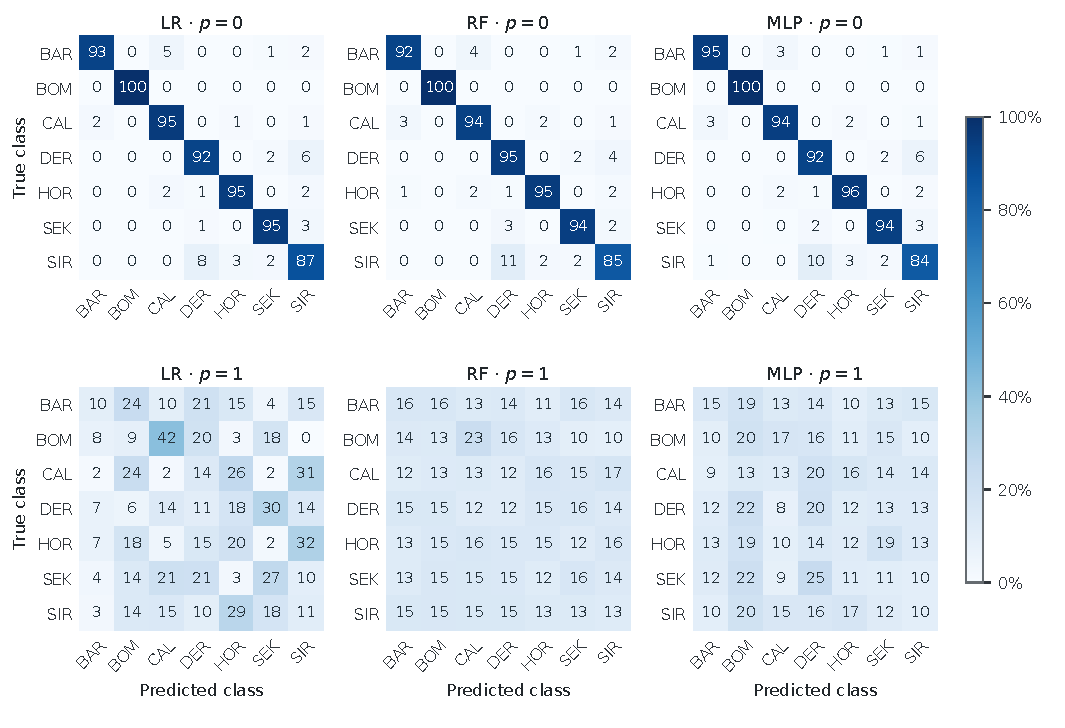
\includegraphics[width=\textwidth]{confusion_endpoints.pdf}
\caption{Row-normalized endpoint confusion matrices. Columns identify LR, RF, and MLP. Top: clean-label training ($p=0$); bottom: complete uniform replacement ($p=1$). Each matrix pools three runs on the same 2,709 unique test observations. Cells show row percentages on a shared 0--100\% scale. Pooling repeated predictions summarizes runs, not additional independent observations.}
\label{fig:confusion}
\end{figure*}

BOMBAY is the smallest training class but is well separated with clean labels: LR recalls all 104 BOMBAY test observations, and RF's mean BOMBAY recall is also 1.0000. Small count alone does not determine class difficulty. For LR, clean-label SIRA F1 is 0.8687, below its seven-class Macro-F1, whereas BOMBAY F1 is 1.0000. The aggregate score therefore does not imply uniform performance across classes.

Complete replacement disrupts diagonal structure. Errors depend on model and seed; low overall performance does not require a uniform prediction histogram. In particular, the large variation in LR's random-label runs argues against selecting one visually striking seed to represent all endpoint behavior. We show aggregated endpoints and retain individual predictions in the reproducible output structure.

\subsection{Optimization and Computation}
Figure~\ref{fig:optimization} relates MLP results to its finite budget. Fourteen of the 15 main MLP runs reach 500 iterations and produce convergence warnings. The clean-label run with seed 17 stops at 430 without that warning; the other two clean-label runs and all twelve randomized runs reach 500. Two MLP candidates also warn during tuning, giving 16 warning-bearing fits among the 55 research fits.

\begin{figure*}[t]
\centering
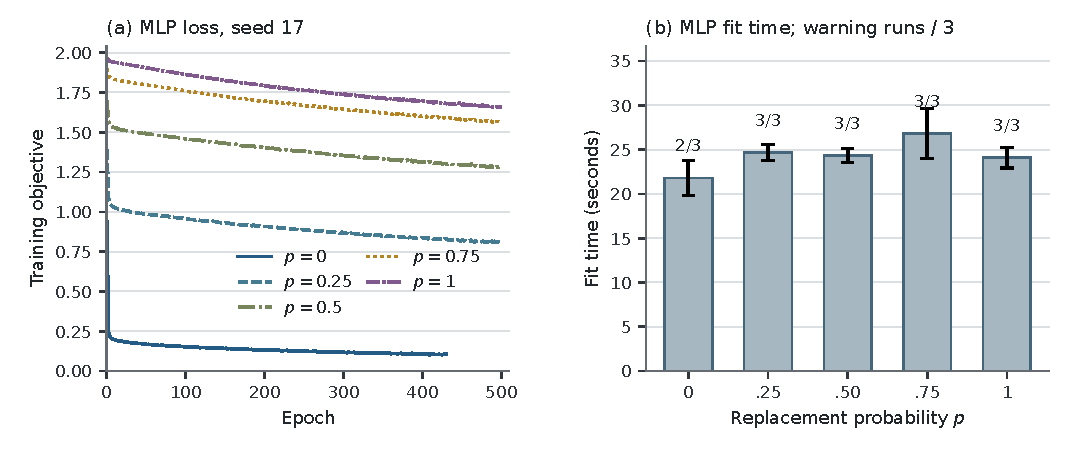
\includegraphics[width=\textwidth]{mlp_optimization.pdf}
\caption{Optimization diagnostics from existing fits. MLP training-objective curves use fixed seed 17 (the first protocol seed) at five noise levels. Different targets define different objectives, so vertical separation is not a clean-test quality comparison. The timing panel uses all 15 MLP main runs, mean $\pm$ sample SD; labels count convergence warnings among three runs per condition. No fitting was performed to generate the figure.}
\label{fig:optimization}
\end{figure*}

We retain every predeclared run instead of silently excluding warnings or extending only unfavorable conditions. A convergence warning does not invalidate saved prediction arithmetic but limits claims about representational capacity or asymptotic optimization. Capacity, L2 regularization, optimizer behavior, and additional iterations cannot be separated without another controlled experiment.

Pure fit time sums to 462.8 seconds across tuning and main experiments, with 401.0 seconds in the main matrix. Main-fit totals are 2.6 seconds for LR, 33.2 for RF, and 365.3 for MLP. These exclude installation, loading, serialization, evaluation, visualization, and inference. Runs use a Windows 11 CPU environment with 20 logical processors, BLAS restricted to one thread during fitting, and four RF workers. The measurements characterize this local execution, not a portable speed benchmark.

\section{Discussion and Limitations}
\label{sec:discussion}
\subsection{Why Partial Noise Can Preserve Signal}
LR's relatively strong result at $p=0.75$ deserves interpretation without a claimed causal explanation. Under independent uniform replacement, let $\eta_k(x)=\Pr(Y=k\mid X=x)$ be the clean population class posterior. The corrupted posterior is
\begin{equation}
\widetilde\eta_k(x)=(1-p)\eta_k(x)+\frac{p}{K}.
\label{eq:posterior}
\end{equation}
For any two classes,
\begin{equation}
\widetilde\eta_a(x)-\widetilde\eta_b(x)
=(1-p)\bigl(\eta_a(x)-\eta_b(x)\bigr).
\end{equation}
For $p<1$, the ordering of ideal population posteriors is preserved, except for existing ties, even though separation shrinks. At $p=1$, all corrupted posteriors equal $1/K$ and no original label signal remains in expectation. This is a direct derivation from our intervention, not an additional empirical result or a theorem attributed to the assigned paper.

Signal retention under substantial replacement is therefore plausible. A restricted model may be less able to follow individual arbitrary assignments while still estimating a useful boundary. However, this does not guarantee finite-sample LR robustness, correct specification, optimization success, or unchanged Macro-F1. Macro-F1 is not the population zero--one-risk objective. Correlated features, imbalance, and regularization all matter. LR's observed behavior invites further explanation; it does not prove that low capacity is universally preferable.

\subsection{Connection to the Assigned Paper}
RF's perfect random-label fitting and poor original-label test prediction illustrate the diagnostic distinction motivating the assigned paper in a different learner and input domain. This observation does not supply a general theory of neural-network generalization.

The MLP result is informative when stated narrowly. Our 128/64 network, selected regularization, and 500-iteration budget do not yield perfect random-label fit. The assigned paper uses different architectures, data, and conditions, and itself reports some random-label fits below 100\%. We neither claim numerical replication nor interpret incomplete fitting as a contradiction. Explicit regularization can affect learning; these experiments do not establish that it is useless or that implicit regularization alone explains all outcomes.

\subsection{Threats to Validity}
\textit{Single dataset and split.} Seeds vary perturbations and initialization on one split. They do not establish sensitivity to new partitions or performance on other tasks. Repeated test predictions are paired observations, not an enlarged independent sample.

\textit{Selection objective.} Parameters are selected on clean labels and held fixed. This makes the intervention interpretable but can disadvantage a model that benefits from noise-specific regularization. Small grids and a finite budget do not equalize effective capacity or exhaustively optimize every family.

\textit{Optimization.} Most MLP fits reach the iteration cap. Loss uses supplied labels, so lower loss cannot be interpreted directly as better original-label prediction. The matrix does not disentangle regularization, size, and optimization.

\textit{Synthetic corruption.} Replacement is feature-independent and can restore an original label by chance. Annotation mistakes may be asymmetric or concentrated near boundaries. The preserved-posterior-order argument does not automatically apply to such mechanisms.

\textit{Uncertainty and post-holdout work.} Sample SD over three runs is descriptive. We conduct no significance tests and do not claim that capacity alone caused a between-model difference. The test results are known; optional larger-network experiments and preprocessing changes remain unrun and would be explicitly exploratory.

\section{Reproducibility and Web Inference}
\label{sec:repro}
\subsection{Repository and Experiment Records}
The implementation uses Python 3.12.14, scikit-learn 1.7.2, NumPy 2.2.6, pandas 2.2.3, SciPy 1.15.3, and Matplotlib 3.10.7. A lock file records transitive versions. Pipeline stages cover preparation, EDA, tuning, training, evaluation, report, and verification. Raw data, configurations, code, tests, summaries, and figures are distinguished from large regenerated artifacts such as models and per-row predictions.

Historical configuration contains a planning-status string that predates execution. Current evidence comes from the final evaluation receipt, per-run metadata, and project ledger. We preserve that history rather than rewrite the timestamped experiment context. A fresh reproduction creates its own environment, freeze record, outputs, and evaluation receipt in a separate workspace. It must not reuse historical seals while claiming a new execution.

On October 18, we exercised that workflow in a new directory and Python environment on the same machine. It repeated all ten tuning and 45 main fits, selected identical parameters, and exactly reproduced every compared non-runtime numerical field in the tuning and main tables. The complete suite passed 47 tests. All six regenerated web models also matched offline probabilities in real local HTTP checks. This validates the documented local workflow; it does not establish cross-platform equivalence. Reproduction timestamps, artifact fingerprints, and runtimes remain separate from the original results.

The repository documentation gives setup and reproduction steps and identifies data attribution. The UCI data carry the stated CC BY 4.0 license. The official IEEE class and bibliography style retain their own notices; no code license is inferred from the dataset license. Large model and prediction files can be regenerated through the documented local pipeline.

Figure assets use saved training data, metric tables, predictions, and optimization records. Vector PDFs and a source manifest allow independent compilation on Overleaf without running the training pipeline. Rebuilding figures is an analysis/rendering operation, not additional research fitting.

\subsection{Hosted and Local Inference Demonstration}
The Flask interface loads six saved Pipelines: one seed-17 model from each family under clean ($p=0$) and fully randomized ($p=1$) supervision. Requests supply 16 numerical inputs in fixed order. Preprocessing remains inside each saved Pipeline, preventing the interface from applying different standardization statistics.

The interface supports model selection, clean/random comparison, editable inputs, and seven-class probability displays. An example's original label appears only while its recorded validation inputs are unchanged; editing features removes that claim. Validation examples are selected by a fixed row-order rule, not prediction correctness. Displayed probabilities are model outputs, not externally calibrated confidence estimates.

Input validation rejects missing or extra fields, nonnumeric or nonfinite values, and extreme magnitudes. Finite values outside training ranges generate a notice rather than silent clipping. Pending requests lock controls until the response arrives, avoiding results displayed under changed selections. The endpoint performs no training and does not read the test partition.

Historical local records show 47 tests passing and restart consistency. The public Vercel Hobby deployment is available at \url{https://ecs171-label-demo.vercel.app}. Anonymous production checks compared all six models on seven validation examples: all 42 predictions matched offline classes and metadata, with maximum probability difference $2.78\times10^{-17}$, below $10^{-12}$. Desktop interaction was checked; full mobile acceptance, a backup recording, and timed rehearsal remain pending.

\section{Conclusion}
\label{sec:conclusion}
In this fixed Dry Bean protocol, randomization separates reproducing supplied training answers from predicting original labels on new observations. RF perfectly fits supplied labels after complete replacement while clean-test Macro-F1 falls to 0.1314. The finite-budget MLP partially fits random labels but also loses useful test performance. LR preserves more clean-test performance at substantial partial replacement in this setting, yet deteriorates sharply when label information is fully removed.

The strongest supported lesson is methodological: state which labels define each metric, preserve the exact corruption mechanism, and evaluate unseen observations against an appropriate reference. Similar clean-label scores can conceal different responses to corrupted supervision. Paired seeds, frozen selection, saved predictions, and reproducible plots make those differences inspectable. Broader rankings, noise-aware optimization, and conclusions about neural-network capacity require experiments beyond the completed matrix.

\clearpage
\balance
\section{Project Roadmap, Contributions, and Availability}
\label{sec:roadmap}
\subsection{Milestones and Completion Evidence}
Table~\ref{tab:roadmap} maps the course workflow to artifacts and remaining work. The technical baseline and public deployment are complete; team acceptance and course submission remain pending. Dates after the proposal deadline are internal targets, subordinate to course announcements and the assigned presentation date.

\begin{table}[h]
\caption{Roadmap snapshot, October 18, 2026.}
\label{tab:roadmap}
\centering\footnotesize
\begin{tabularx}{\columnwidth}{@{}L{0.95in}X@{}}
\toprule
Milestone & Status / evidence or next deliverable\\
\midrule
Paper and problem & Complete: paper reviewed; RQ1/RQ2 and noise protocol specified.\\
Literature review & Core references checked for this report; team review pending.\\
Dataset and EDA & Complete: source archive, audit, fixed split, training-only EDA.\\
Preprocessing & Complete: 16 features; train-fitted scaling for LR/MLP.\\
Development / tuning & Complete: ten clean candidates; settings frozen.\\
Main experiments & Complete: 45 fits, predictions, warnings, and time records.\\
Evaluation & Complete: predeclared clean holdout; 15 condition summaries.\\
Web demo & Vercel production live; anonymous inference verified; backup video pending.\\
Proposal, Oct. 21 & One-page LaTeX/PDF prepared; team confirmation and submission pending.\\
Mid-quarter, Oct. 28 & Three-page draft prepared; internal team-review target.\\
Report / repo, Nov.~4 & Internal target: team-accepted report and documented repository release.\\
Presentation, Nov.~11 & Internal target: delivery check and five-minute rehearsal.\\
\bottomrule
\end{tabularx}
\end{table}

\subsection{Responsibilities and Contribution Record}
The planned division names Linjie Yang as technical lead for validation, analysis, reproducibility, inference integration, and drafting; Tianying Chen as team leader for coordination, interface acceptance, and submission organization; and Elsey Chen for dataset/reference checks and independent figure/metric review. These roles remain subject to team confirmation.

The execution record identifies local implementation and experiment runs as performed with Codex assistance under Linjie Yang's instructions. This report and repository preparation likewise use that assistance. The record does not independently establish completed contributions by the other members. Each member should review the outputs and record actual tasks, review notes, and attributable commits before final submission. Planned assignments are not presented as completed individual contributions.

\subsection{Code and Artifact Availability}
The source repository is
\begin{center}
\footnotesize
\url{https://github.com/Felix-Yang-369/ecs171-label-randomization}.
\end{center}
It is private at preparation time; instructor and teammate access must be arranged before assessment. It contains the implementation, environment instructions, experiment summaries, and this paper's LaTeX source. Large model and prediction artifacts are regenerated through the documented pipeline rather than assumed present after cloning. The paper package includes finished figure assets for independent compilation.

The pre-report snapshot is commit \code{1d19a2a}; later documentation and deployment work preserve frozen training sources and results. Hosting uses the existing free Hobby plan, without paid integrations. The README and reproduction guide are entry points. Presentation allocation, contribution sign-off, and course submission remain to be confirmed.

\clearpage
\nobalance
\bibliographystyle{IEEEtran}
\bibliography{references}
\end{document}
